\documentclass[tikz,margin=0pt,dvipsnames,rgb]{standalone}

\usepackage{amsmath,amssymb,amsfonts}
\usetikzlibrary{calc,
fit,
shapes.misc,
shapes.geometric,
arrows.meta,
fadings,
matrix,
chains,
scopes,
positioning}

\usepackage{pgfplots}
\usepackage{pgfplotstable}
\pgfplotsset{compat=1.18}



\usepackage[]{fontspec}

\setmainfont{Latin Modern Roman}
\setmonofont{Latin Modern Math}
\renewcommand{\textsc}[1]{{\fontfamily{lmr}\selectfont \scshape #1}}

\usepackage[]{bm}

\makeatletter
\@ifundefined{fromRoot}{\newcommand{\fromRoot}[1]{../../#1}}{}

\def\input@path{{../..}{..}{.}{./svg}{./pgfplots}{./tikzpicture}}
%or: \def\input@path{{/path/to/folder/}{/path/to/other/folder/}}
\makeatother

\newcommand*{\gf}[1]{\acrshort{gf}($#1$)}%
\newcommand*{\mpn}[1]{\bm{P}_{#1}}%
\newcommand*{\pn}[1]{%
  \ifthenelse{\equal{#1}{}}{$\mpn{0}$}{$\mpn{#1}$}%
}%

\newcommand*{\pk}[3]{%
  \ifthenelse{\equal{#1}{#2}}{\textcolor{red}{\phantom{.}$p_0$\phantom{.}}}{\phantom{.}$p_#3$\phantom{.}}%
}%


\newcommand*{\placeholder}{
\includegraphics[width=\linewidth, height=.25\textheight, keepaspectratio = true]{figures/certified_xilinx.png}}%

\newcommand*{\snr}{\acrshort{snr}}%
\newcommand*{\snrs}{\acrshortpl{snr}}%

\newcommand*{\mpd}[0]{p_\Delta}%
\newcommand*{\mpo}[0]{p_\omega}%
\newcommand*{\pd}[0]{$\mpd$}%
\newcommand*{\po}[0]{$\mpo$}%
\newcommand*{\mpfa}[0]{\mathcal{P}_{fa}}%
\newcommand*{\mpmd}[0]{\mathcal{P}_{md}}%
\newcommand*{\pfa}[0]{\acrshort{pfa}}%
\newcommand*{\pmd}[0]{\acrshort{pmd}}%
\newcommand*{\mnorm}[1]{\mathcal{L}_{#1}}%
\newcommand*{\norm}[1]{$\mnorm{#1}$}%
\newcommand*{\fft}{\acrshort{fft}}%
\newcommand*{\mfft}[1]{\mathcal{F}(#1)}%
\newcommand*{\mifft}[1]{\mathcal{F}^{-1}(#1)}%
\newcommand*{\ts}{\acrshort{ts}}%

\newcommand*{\cpp}[1]{C\textrm{++#1}}%
\newcommand*{\na}{\textrm{\textcolor{SlateGray4}{N/A}}}%

\newcommand*{\vect}[1]{\bm{#1}}%
\newcommand*{\mat}[1]{\bm{\mathrm{#1}}}%

\newcommand*{\task}[1]{\mathcal{T}_{#1}}%

\newcommand*{\sdr}{\acrshort{sdr}}%
\newcommand*{\fpga}{\acrshort{fpga}}%



\DeclareMathSymbol{\shortminus}{\mathbin}{AMSa}{"39}

\begin{document}

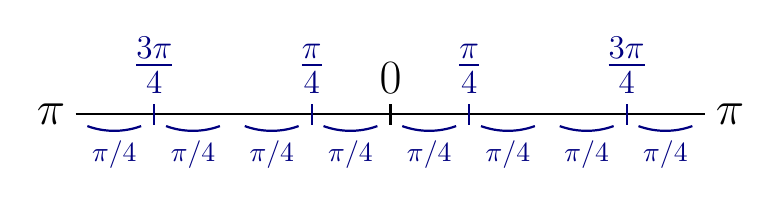
\begin{tikzpicture}[
    thick,
    every node/.style={font=\LARGE},
  ]
  \node [anchor=east]         (mpi) at (-4, 0) {$\shortminus\pi$};
  \node [anchor=west]         (ppi) at (+4, 0) {$\pi\phantom{\shortminus}$};
  \node [label = {above:$0$}] (z)   at ( 0, 0) {};

  % \node[label = {above:\textcolor{DarkOrchid}{$\shortminus\frac{\pi}{2}\phantom{\shortminus}$}}] (mpo2) at (-2, 0) {};
  % \node[label = {above:\textcolor{DarkOrchid}{$\frac{\pi}{2}$}}]  (ppo2) at (+2, 0) {};

  \node[label = {above:\textcolor{NavyBlue}{$\shortminus\frac{3\pi}{4}\phantom{\shortminus}$}}] (m3po4) at (-3, 0) {};
  \node[label = {above:\textcolor{NavyBlue}{$\shortminus\frac{ \pi}{4}\phantom{\shortminus}$}}]  (m1po4) at (-1, 0) {};
  \node[label = {above:\textcolor{NavyBlue}{$\frac{\pi}{4}$}}]   (p1po4) at (+1, 0) {};
  \node[label = {above:\textcolor{NavyBlue}{$\frac{3\pi}{4}$}}]  (p3po4) at (+3, 0) {};

  \draw [-] (mpi.east) -- (ppi.west);
  \draw [-, thick] (z.south) -- (z.north);

  % \draw [-, thick, DarkOrchid] (mpo2.south) -- (mpo2.north);
  % \draw [-, thick, DarkOrchid] (ppo2.south) -- (ppo2.north);

  \draw [-, thick, NavyBlue] (m3po4.south) -- (m3po4.north);
  \draw [-, thick, NavyBlue] (m1po4.south) -- (m1po4.north);
  \draw [-, thick, NavyBlue] (p1po4.south) -- (p1po4.north);
  \draw [-, thick, NavyBlue] (p3po4.south) -- (p3po4.north);

  % \draw[DarkOrchid, thick] (4, 0) arc[start angle=65, end angle=115, radius=1cm];

  \foreach \i in {-4, -2, 0, 2} {
    \draw[draw=none,  thick] (\i, -.15)+(.15, 0) arc[start angle=-110, end angle=-70, radius=2.45cm]
    node [midway, below, font=\normalsize] {\phantom{$\pi/2$}};
  }
  \foreach \i in {-4, -3, -2, -1, 0, 1, 2, 3} {
      \draw[NavyBlue, thick] (\i, -.15)+(.15, 0) arc[start angle=-110, end angle=-70, radius=1.cm]
      node [midway, below, font=\normalsize] {$\pi/4$};
    }

\end{tikzpicture}

\end{document}
